\documentclass{beamer}
\usetheme{Berkeley}
\usecolortheme[RGB={132,184,24}]{structure} 
\usepackage[utf8x]{inputenc}
\usepackage{ucs}
\usepackage{amsmath}
\usepackage{amsfonts}
\usepackage{amssymb}
\usepackage{enumerate}
\usepackage{listings}
\logo{\pgfimage[width=15.7mm]{tudo127x97.jpg}}
\title{Einführung WS11/12}
\begin{document}

\section{Willkommen}
\begin{frame}{Willkommen}
\begin{center}
\huge
WebTech I - Blatt 2
\vspace{7mm}
\pgfimage[width=7cm]{ringe.jpg}

\end{center}
\end{frame}

\begin{frame}{Einführung}
\begin{center}Thema: JavaScript und DOM-Scripting\end{center}
\begin{itemize}
\item Aufgabe 2.1: Clientseitige Formularvalidierung
\item Aufgabe 2.2: Dynamisches Erweitern von HTML-Dokumenten
\item Aufgabe 2.3: Tooltip-Fenster
\item Aufgabe 2.4: Tabellenzeilen in JavaScript dynamisch hervorheben
\end{itemize}
\end{frame}

\begin{frame}{Aufgabe 2.1}
\begin{center}
Implementierung einer clientseitigen Formularvalidierung mithilfe von JavaScript (innerhalb der HTML-Datei):\\
~\\~\\
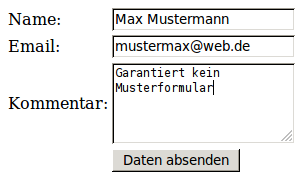
\includegraphics[width = 120px]{A1/src/formvali.png}
\\
Betrachtet werden die für die Aufgabe relevanten $\langle${\bf form}$\rangle$ - und $\langle${\bf script}$\rangle$ -Tags:
\end{center}
\end{frame}

\tiny{
\begin{lstlisting}[language = HTML,
				   mathescape = true, 
                   morekeywords = {onsubmit, onclick, this, return}, 
                   numbers = left, 
                   numbersep = 3pt]
 <form name = "vali" method = "post" action = "aufgabe2_1.html"
 onsubmit = "return$~$validate(this);">
<table border= "0" cellpadding= "0" cellspacing= "4">
 <tr>
  <td align = "left">Name:</td>
  <td align = "left">
  <input type = "text" name = "nameTextField" size = "20"></td>
 </tr>
 <tr>
  <td align = "left">Email:</td>
  <td align = "left">
  <input type = "text" name = "eMailTextField" size = "20"></td>
 </tr>
 <tr>
  <td align = "left">Kommentar:</td>
  <td align = "left">
  <textarea name = "commentTextArea" rows = "4" cols = "15">
  </textarea></td>
 </tr>
 <tr>
  <td align = "left"></td>
  <td align = "left">
  <input type = "button" value = "Daten$~$absenden" name = "validateButton" 
   onclick = "validate(this);"></td>
 </tr>
</table>
</form>
\end{lstlisting}}

\begin{frame}{javascript}
\end{frame}
\end{document}
